\documentclass{article}

\pdfminorversion=4

\usepackage{fullpage}
\usepackage{tikz}
\usetikzlibrary{fit}

\def\DeflateHeader{\begingroup
  \pdfcompresslevel=0\relax
  \pdfobjcompresslevel=0\relax
    \immediate\pdfobj stream
        file {.DEFLATEDummyHeader}
\endgroup}

\def\DeflateHeaderObj{\begingroup
  \pdfcompresslevel=0\relax
  \pdfobjcompresslevel=0\relax
    {\catcode`\%=12\immediate\pdfliteral{%RRRRR
}}\endgroup}

\begin{document}

\title{This PDF is a Git Repository\\Containing its Own \LaTeX\ Source}
\author{Evan Sultanik}
\date{April 11, 2017}

\maketitle

Have you ever heard of the \texttt{git bundle} command? I hadn't. It
bundles a set of Git objects---potentially even an entire
repository---into a single file. Git allows you to treat that file as
if it were a standard Git database, so you can do things like clone a
repo directly from it. Its purpose is to easily sneakernet pushes or
even whole repositories across air gaps.

The file format for Git bundles doesn't appear to be formally
specified anywhere, however, inspecting \texttt{bundle.c} reveals that
it's relatively straightforward:
\begin{center}
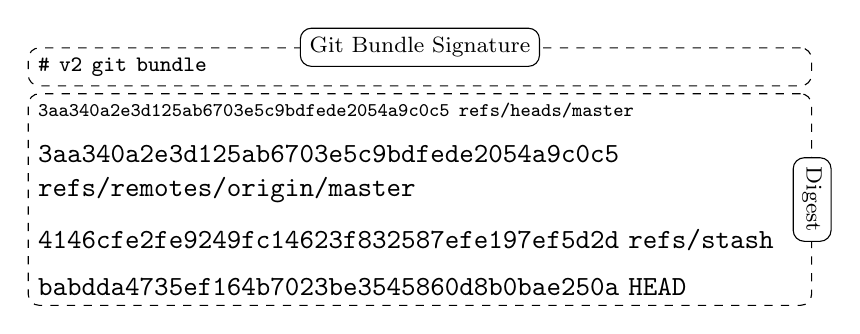
\begin{tikzpicture}
  \node[text width=0.8\hsize] at (0,0) (sig) {\footnotesize\texttt{\# v2 git bundle}};
  \node[inner sep=0mm,fit=(sig),draw,rounded corners,dashed,minimum width=0.8\hsize] (sigbox) {};
  \node[draw,rounded corners,fill=white] at (sigbox.north) (siglabel) {\footnotesize Git Bundle Signature};
  \node[text width=0.8\hsize,anchor=north west,yshift=-1mm] at (sig.south west) (b1) {\scriptsize\tt 3aa340a2e3d125ab6703e5c9bdfede2054a9c0c5 refs/heads/master};
  \node[text width=0.8\hsize,anchor=north west,yshift=-1mm] at (b1.south west) (b2) {\tt 3aa340a2e3d125ab6703e5c9bdfede2054a9c0c5 refs/remotes/origin/master};
  \node[text width=0.8\hsize,anchor=north west,yshift=-1mm] at (b2.south west) (b3) {\tt 4146cfe2fe9249fc14623f832587efe197ef5d2d refs/stash};
  \node[text width=0.8\hsize,anchor=north west,yshift=-1mm] at (b3.south west) (b4) {\tt babdda4735ef164b7023be3545860d8b0bae250a HEAD};
  \node[inner sep=0mm,fit=(b1) (b4),draw,rounded corners,dashed,minimum width=0.8\hsize] (digestbox) {};
  \node[rotate=-90,draw,rounded corners,fill=white] at (digestbox.east) {\footnotesize Digest};
\end{tikzpicture}
\end{center}

\end{document}
